%!TEX program = xelatex
\documentclass[9pt, compress]{beamer}
\usetheme[titleprogressbar]{m}

\usepackage{array}
\usepackage{tabu}
\usepackage{longtable} %tabu needs this to be loaded.
\usepackage{lipsum}
\usepackage{multicol}
\usepackage{rotating}

\usepackage{color}
\usepackage{xcolor}
\usepackage{listings}
\usepackage{sectsty}
\usepackage{caption}


\DeclareCaptionFont{white}{\color{white}}
\DeclareCaptionFormat{listing}{\colorbox{gray}{\parbox{\dimexpr\textwidth-1.72\fboxsep\relax}{#1#2#3}}}
\captionsetup[lstlisting]{format=listing,labelfont=white,textfont=white,margin=0pt}
\lstset{language=C,
	basicstyle=\footnotesize,
	keepspaces=true,
	tabsize=4,               
	frame=single,                           % Single frame around code
	rulecolor=\color{black},
	captionpos=b,
	showstringspaces=false,	
	abovecaptionskip=-0.9pt,
	xleftmargin=3.4pt,
	xrightmargin=2.6pt,
	breaklines=true,
	postbreak=\raisebox{0ex}[0ex][0ex]{\ensuremath{\color{black}\hookrightarrow\space}},
	xleftmargin=3.2pt,
	escapechar=\&,
	literate={а}{{\selectfont\char224}}1
	{~}{{\textasciitilde}}1
	{б}{{\selectfont\char225}}1
	{в}{{\selectfont\char226}}1
	{г}{{\selectfont\char227}}1
	{д}{{\selectfont\char228}}1
	{е}{{\selectfont\char229}}1
	{ё}{{\"e}}1
	{ж}{{\selectfont\char230}}1
	{з}{{\selectfont\char231}}1
	{и}{{\selectfont\char232}}1
	{й}{{\selectfont\char233}}1
	{к}{{\selectfont\char234}}1
	{л}{{\selectfont\char235}}1
	{м}{{\selectfont\char236}}1
	{н}{{\selectfont\char237}}1
	{о}{{\selectfont\char238}}1
	{п}{{\selectfont\char239}}1
	{р}{{\selectfont\char240}}1
	{с}{{\selectfont\char241}}1
	{т}{{\selectfont\char242}}1
	{у}{{\selectfont\char243}}1
	{ф}{{\selectfont\char244}}1
	{х}{{\selectfont\char245}}1
	{ц}{{\selectfont\char246}}1
	{ч}{{\selectfont\char247}}1
	{ш}{{\selectfont\char248}}1
	{щ}{{\selectfont\char249}}1
	{ъ}{{\selectfont\char250}}1
	{ы}{{\selectfont\char251}}1
	{ь}{{\selectfont\char252}}1
	{э}{{\selectfont\char253}}1
	{ю}{{\selectfont\char254}}1
	{я}{{\selectfont\char255}}1
	{А}{{\selectfont\char192}}1
	{Б}{{\selectfont\char193}}1
	{В}{{\selectfont\char194}}1
	{Г}{{\selectfont\char195}}1
	{Д}{{\selectfont\char196}}1
	{Е}{{\selectfont\char197}}1
	{Ё}{{\"E}}1
	{Ж}{{\selectfont\char198}}1
	{З}{{\selectfont\char199}}1
	{И}{{\selectfont\char200}}1
	{Й}{{\selectfont\char201}}1
	{К}{{\selectfont\char202}}1
	{Л}{{\selectfont\char203}}1
	{М}{{\selectfont\char204}}1
	{Н}{{\selectfont\char205}}1
	{О}{{\selectfont\char206}}1
	{П}{{\selectfont\char207}}1
	{Р}{{\selectfont\char208}}1
	{С}{{\selectfont\char209}}1
	{Т}{{\selectfont\char210}}1
	{У}{{\selectfont\char211}}1
	{Ф}{{\selectfont\char212}}1
	{Х}{{\selectfont\char213}}1
	{Ц}{{\selectfont\char214}}1
	{Ч}{{\selectfont\char215}}1
	{Ш}{{\selectfont\char216}}1
	{Щ}{{\selectfont\char217}}1
	{Ъ}{{\selectfont\char218}}1
	{Ы}{{\selectfont\char219}}1
	{Ь}{{\selectfont\char220}}1
	{Э}{{\selectfont\char221}}1
	{Ю}{{\selectfont\char222}}1
	{Я}{{\selectfont\char223}}1,
	extendedchars=true
}
\usepackage{textpos}
\newcommand<>{\fullsizegraphic}[1]{
  \begin{textblock*}{0cm}(-0.9cm,-3.78cm)
  \includegraphics[width=\paperwidth]{#1}
  \end{textblock*}
}

%галочка
\usepackage{amssymb}% http://ctan.org/pkg/amssymb
\usepackage{pifont}% http://ctan.org/pkg/pifont
\newcommand{\cmark}{\ding{52}}%
\newcommand{\xmark}{\ding{56}}

\usepackage{booktabs}  
\usepackage[scale=2]{ccicons}
\usepackage{minted}
\usepgfplotslibrary{dateplot}
\usemintedstyle{trac}
\author{Студент: \textbf{Д.В. Круминьш}\\ 
	Группа: \textbf{13541/3}\\ \\
	Преподаватель: \textbf{И.А. Малышев} } 
\title{Отчет о лабораторной работе №5}
\subtitle{Курс: \textbf{Администрирование компьютерных сетей}\\
Тема: \textbf{Перенос сети в Cisco Packet Tracer}}
%\logo{123}
\institute{Санкт-Петербургский политехнический университет Петра Великого}
\date{ }
%\subject{}
%\setbeamercovered{transparent}
%\setbeamertemplate{navigation symbols}{}
\begin{document}
	\maketitle
%	\begin{frame}
%		\frametitle{Оглавление}
%		\tableofcontents{}
	%\end{frame}
\begin{frame}
\frametitle{Цели работы}
\begin{enumerate}
\item Ознакомиться с Cisco Packet Tracer, и выполнить в нем:
\begin{itemize}
\item Построение компьютерной сети(из прошлых работ);
\item Настроить сервисы DNS, DHCP, TFTP;
\item Выполнить тестирование сети.
\end{itemize}
\end{enumerate}
\end{frame}

\section{Построение компьютерной сети}

\begin{frame}
\frametitle{Общая схема компьютерной сети}
\begin{center}  
	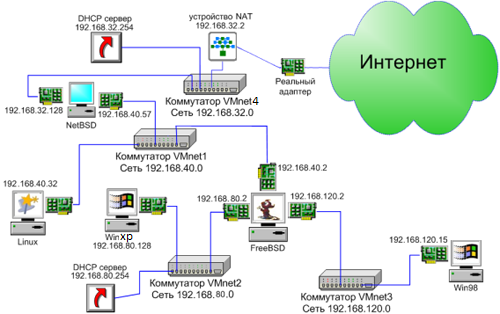
\includegraphics[width=\textwidth]{img/KKS_full}
\end{center}
\end{frame}


\begin{frame}
\frametitle{Пояснения к схеме}
Средствами Cisco Packet Tracer будет построена схема, из слайда ранее, за следующим исключением:
\begin{itemize}
\item Вместо NetBSD и FreeBSD будут использоваться роутеры;
\item Вместо интернета будет выступуать сервер с http страницой.
\end{itemize}
С помощью инструментов, были расставлены компьютеры, коммутаторы и роутеры типа \textbf{generic}, а также связаны между собой.

Дополнительно, узлам были расставлены текстовые метки, где указан их адрес, а также сервисы данного узла.
\end{frame}


\begin{frame}
\frametitle{Схема компьютерной сети в CISCO}
\begin{center}  
	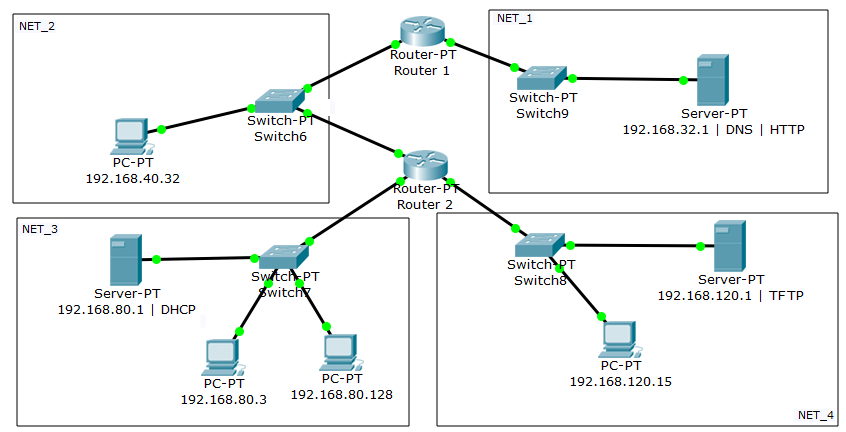
\includegraphics[width=\textwidth]{img/my_kks}
\end{center}
\end{frame}


\begin{frame}
\frametitle{Пояснения к дальнейшей настройке}
Далее приведена настройка каждого узла, заголовок слайдов будет выполнен в следующем стиле:
\begin{center}
\textbf{Настройка <название сети> | <адрес узла>}
\end{center}
или
\begin{center}
\textbf{Настройка <название роутера>}
\end{center}
Где:
\begin{itemize}
\item \textbf{<название сети>} - одно из возможных названий сети(NET\_1, NET\_2, NET\_3, NET\_4);
\item \textbf{адрес узла} - адрес узла принадлежащий выбранной сети;
\item \textbf{название роутера} - одно из возможных названий роутера(Router 1, Router 2).
\end{itemize}
Коммутаторы в настройке не требуются.
\end{frame}


\begin{frame}
\frametitle{Настройка NET\_1 | 192.168.32.1}
Установка статического адреса, и указания самого себя в качестве DNS сервера.
\begin{center}  
	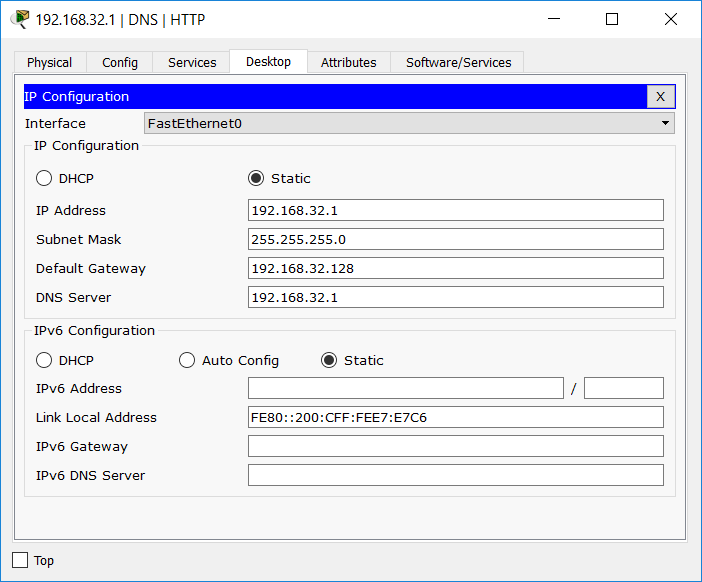
\includegraphics[width=.7\textwidth]{img/192_168_32_1__0}
\end{center}
\end{frame}

\begin{frame}
\frametitle{Настройка NET\_1 | 192.168.32.1}
Добавленная DNS запись для \textbf{www.mypage.com} на адрес 192.168.32.1.
\begin{center}  
	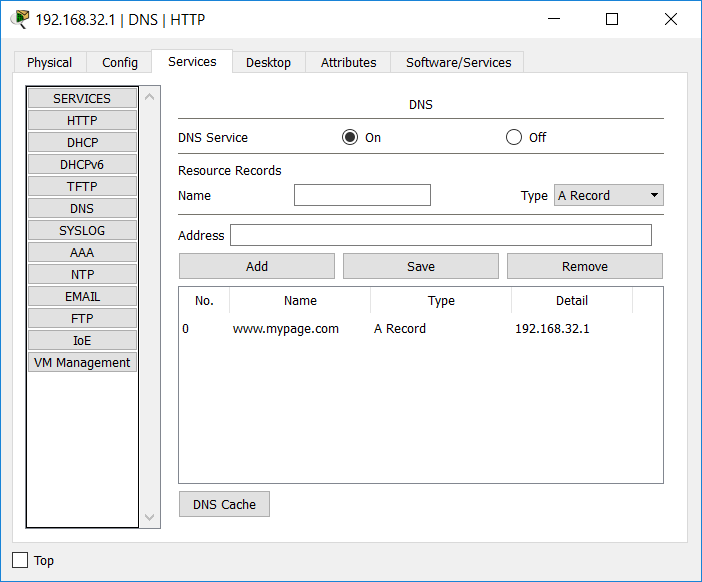
\includegraphics[width=.7\textwidth]{img/192_168_32_1__1}
\end{center}
\end{frame}


\begin{frame}
\frametitle{Настройка Router 1}
Указание статического адреса \textbf{192.168.32.128} для интерфейса \textbf{FastEthernet0/0}, для сети NET\_1.
\begin{center}  
	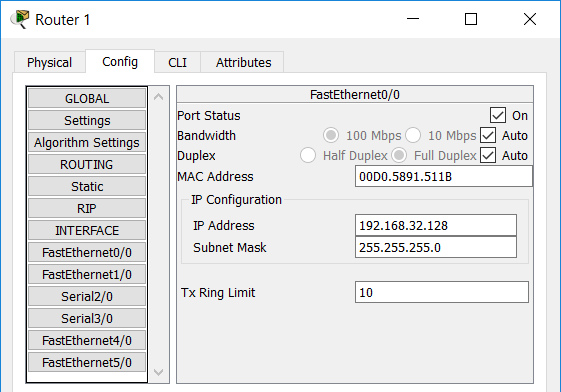
\includegraphics[width=.8\textwidth]{img/router_1__0}
\end{center}
\end{frame}

\begin{frame}
\frametitle{Настройка Router 1}
Указание статического адреса \textbf{192.168.40.57} для интерфейса \textbf{FastEthernet1/0}, для сети NET\_2.
\begin{center}  
	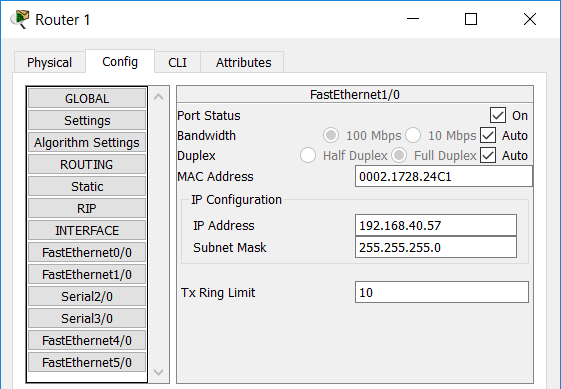
\includegraphics[width=.8\textwidth]{img/router_1__1}
\end{center}
\end{frame}

\begin{frame}
\frametitle{Настройка Router 1}
Добавление маршрутизацию для сетей \textbf{192.168.40.0} и \textbf{192.168.32.0}.
\begin{center}  
	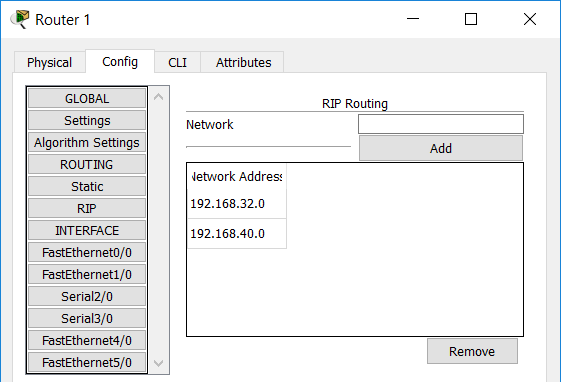
\includegraphics[width=.8\textwidth]{img/router_1__2}
\end{center}
\end{frame}


\begin{frame}
\frametitle{Настройка NET\_2 | 192.168.40.32}
Установка статического адреса, шлюза(роутер) и DNS сервера.
\begin{center}  
	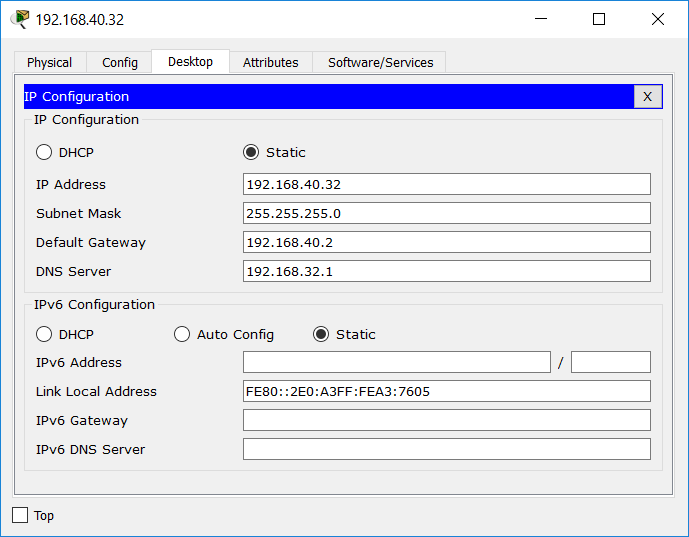
\includegraphics[width=.7\textwidth]{img/192_168_40_32__0}
\end{center}
\end{frame}


\begin{frame}
\frametitle{Настройка Router 2}
Указание статического адреса \textbf{192.168.80.2} для интерфейса \textbf{FastEthernet0/0}, для сети NET\_3.
\begin{center}  
	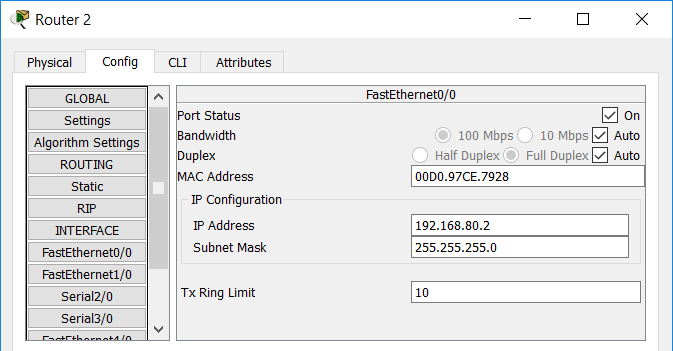
\includegraphics[width=.8\textwidth]{img/router_2__0}
\end{center}
\end{frame}

\begin{frame}
\frametitle{Настройка Router 2}
Указание статического адреса \textbf{192.168.40.2} для интерфейса \textbf{FastEthernet1/0}, для сети NET\_2.
\begin{center}  
	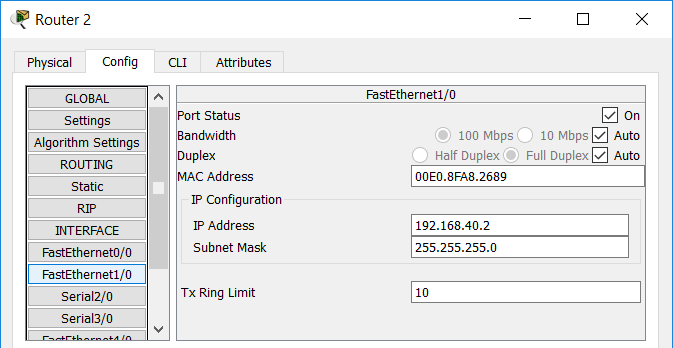
\includegraphics[width=.8\textwidth]{img/router_2__1}
\end{center}
\end{frame}

\begin{frame}
\frametitle{Настройка Router 2}
Указание статического адреса \textbf{192.168.120.2} для интерфейса \textbf{FastEthernet6/0}, для сети NET\_4.
\begin{center}  
	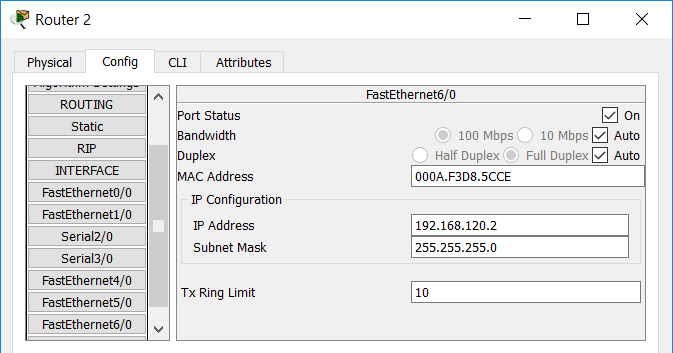
\includegraphics[width=.8\textwidth]{img/router_2__2}
\end{center}
\end{frame}

\begin{frame}
\frametitle{Настройка Router 2}
Добавление маршрутизацию для сетей \textbf{192.168.40.0}, \textbf{192.168.80.0} и \textbf{192.168.120.0}.
\begin{center}  
	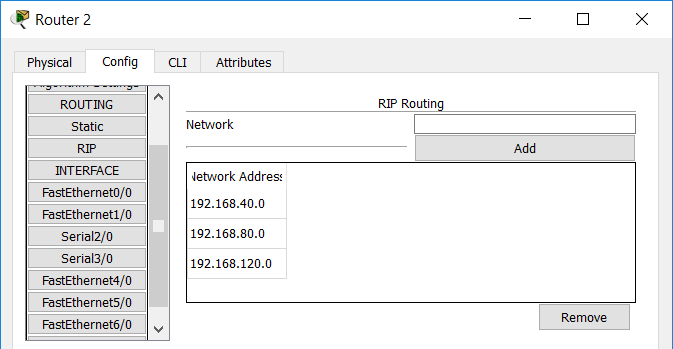
\includegraphics[width=.8\textwidth]{img/router_2__3}
\end{center}
\end{frame}


\begin{frame}
\frametitle{Настройка NET\_3 | 192.168.80.1}
Установка статического адреса, шлюза и DNS сервера.
\begin{center}  
	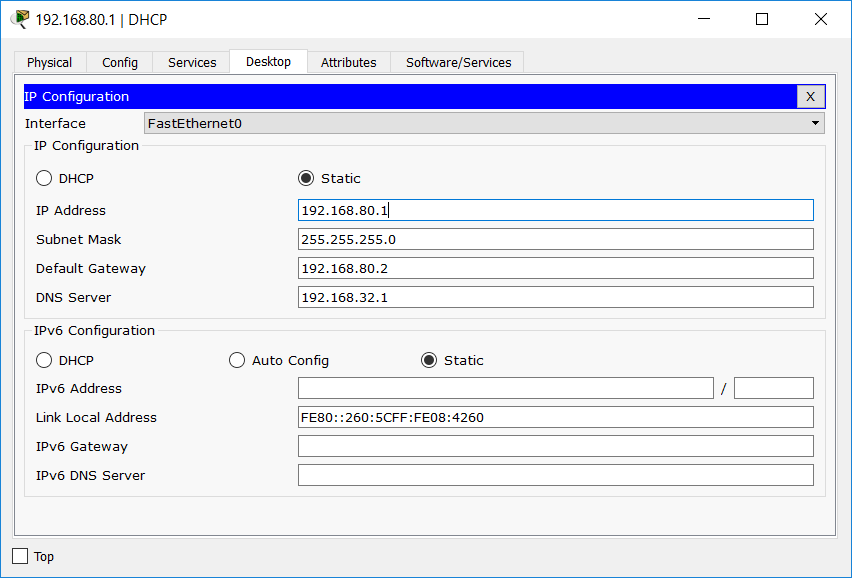
\includegraphics[width=.7\textwidth]{img/192_168_80_1__0}
\end{center}
\end{frame}

\begin{frame}
\frametitle{Настройка NET\_3 | 192.168.80.1}
Настройка DHCP, диапазон адресов начинается с 192.168.80.3.
\begin{center}  
	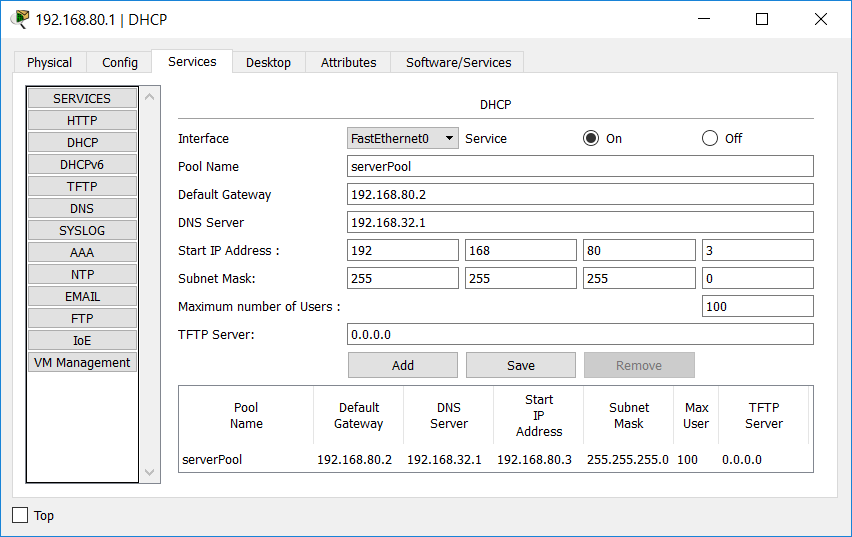
\includegraphics[width=.9\textwidth]{img/192_168_80_1__1}
\end{center}
\end{frame}


\begin{frame}
\frametitle{Настройка NET\_3 | 192.168.80.3}
Адрес был получен автоматически, с помощью сервера DHCP.
\begin{center}  
	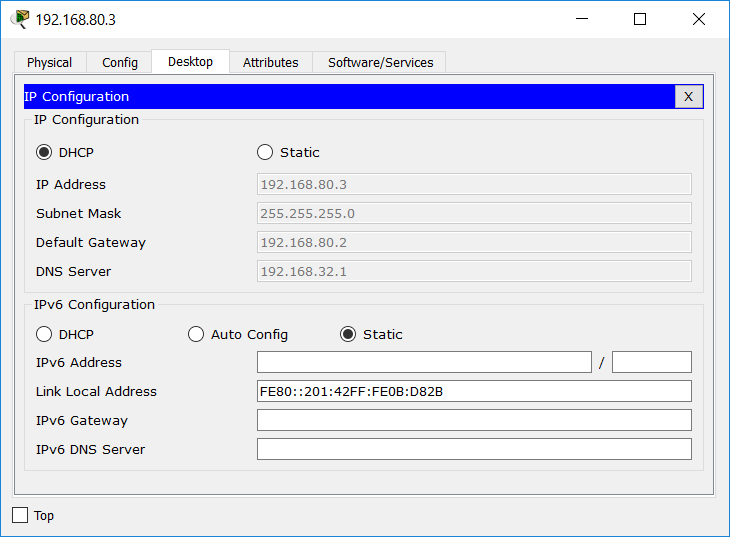
\includegraphics[width=.7\textwidth]{img/192_168_80_3__0}
\end{center}
\end{frame}


\begin{frame}
\frametitle{Настройка NET\_3 | 192.168.80.128}
Установка статического адреса, шлюза и DNS сервера.
\begin{center}  
	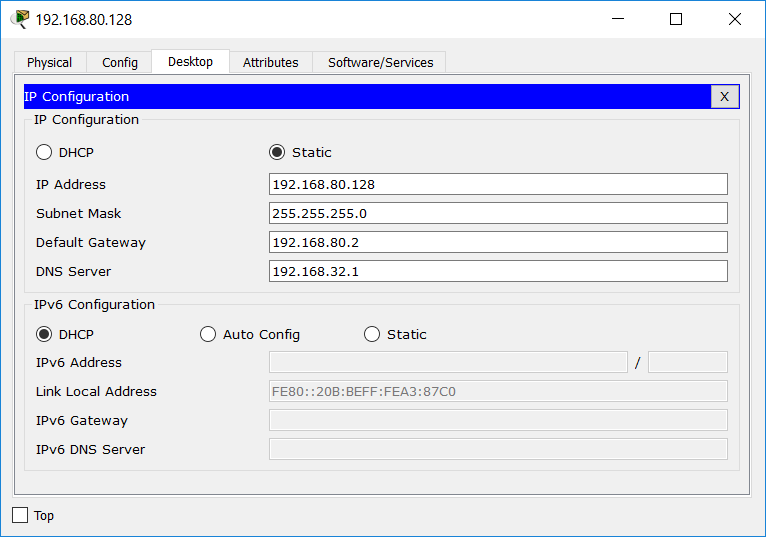
\includegraphics[width=.8\textwidth]{img/192_168_80_128__0}
\end{center}
\end{frame}


\begin{frame}
\frametitle{Настройка NET\_4 | 192.168.120.15}
Установка статического адреса, шлюза и DNS сервера.
\begin{center}  
	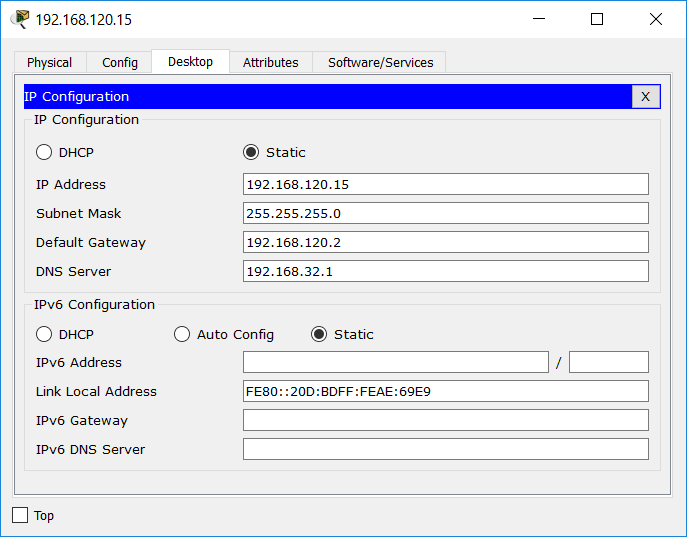
\includegraphics[width=.8\textwidth]{img/192_168_120_15__0}
\end{center}
\end{frame}


\begin{frame}
\frametitle{Настройка NET\_4 | 192.168.120.1}
Установка статического адреса, шлюза и DNS сервера.
\begin{center}  
	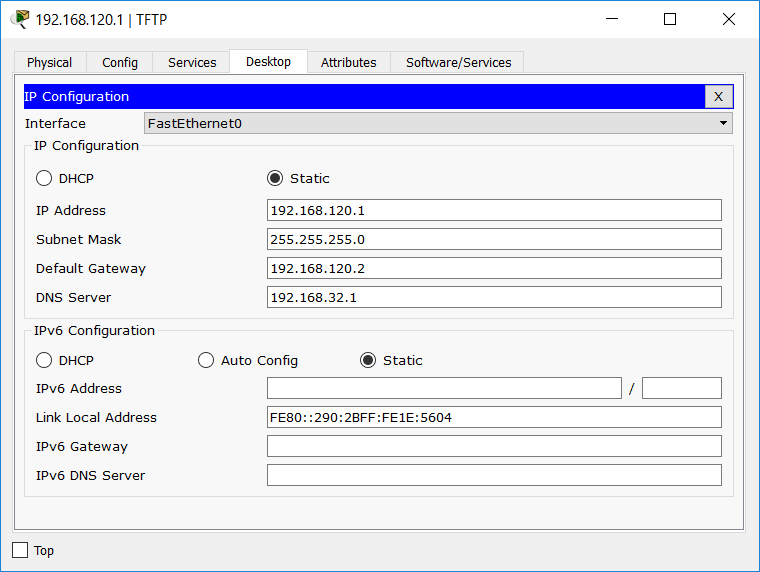
\includegraphics[width=.8\textwidth]{img/192_168_120_1__0}
\end{center}
\end{frame}


\begin{frame}
\frametitle{Настройка NET\_4 | 192.168.120.1}
Включение TFTP сервиса и удаления всех, стандартных файлов на нем.
\begin{center}  
	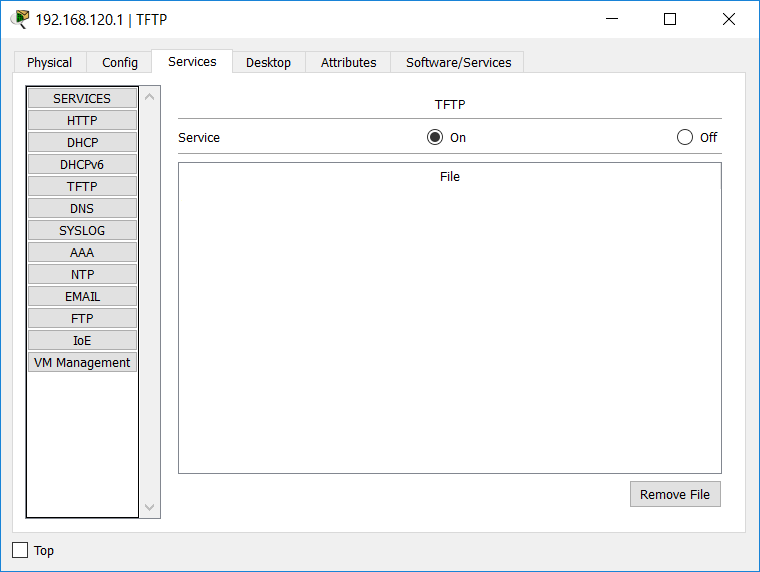
\includegraphics[width=.8\textwidth]{img/192_168_120_1__1}
\end{center}
\end{frame}

\section{Тестирование}

\begin{frame}[fragile]
\frametitle{Проверка команды ping по адресу}
\begin{lstlisting}[language={}]
C:\>ipconfig
FastEthernet0 Connection:(default port)
   Link-local IPv6 Address.........: FE80::2E0:A3FF:FEA3:7605
   IP Address......................: 192.168.40.32
   Subnet Mask.....................: 255.255.255.0
   Default Gateway.................: 192.168.40.2

C:\>ping 192.168.120.15
Pinging 192.168.120.15 with 32 bytes of data:
Reply from 192.168.120.15: bytes=32 time=1ms TTL=127
Reply from 192.168.120.15: bytes=32 time=1ms TTL=127
Reply from 192.168.120.15: bytes=32 time=1ms TTL=127
Reply from 192.168.120.15: bytes=32 time<1ms TTL=127

Ping statistics for 192.168.120.15:
    Packets: Sent = 4, Received = 4, Lost = 0 (0% loss),
Approximate round trip times in milli-seconds:
    Minimum = 0ms, Maximum = 1ms, Average = 0ms
\end{lstlisting}
Успешный пинг узла 192.168.120.15(сеть NET\_4) из сети NET\_2 узлом 192.168.40.32. 
\end{frame}


\begin{frame}[fragile]
\frametitle{Проверка команды ping по доменному имени}
\begin{lstlisting}[language={}]
C:\>ipconfig
FastEthernet0 Connection:(default port)
   Link-local IPv6 Address.........: FE80::201:42FF:FE0B:D82B
   IP Address......................: 192.168.80.3
   Subnet Mask.....................: 255.255.255.0
   Default Gateway.................: 192.168.80.2

C:\>ping www.mypage.com
Pinging 192.168.32.1 with 32 bytes of data:
Reply from 192.168.32.1: bytes=32 time<1ms TTL=126
Reply from 192.168.32.1: bytes=32 time=10ms TTL=126
Reply from 192.168.32.1: bytes=32 time=11ms TTL=126
Reply from 192.168.32.1: bytes=32 time=13ms TTL=126

Ping statistics for 192.168.32.1:
    Packets: Sent = 4, Received = 4, Lost = 0 (0% loss),
Approximate round trip times in milli-seconds:
    Minimum = 0ms, Maximum = 13ms, Average = 8ms
\end{lstlisting}
Успешный пинг узла 192.168.32.1(сеть NET\_1, домен mypage.com) из сети NET\_3 узлом 192.168.80.3. 
\end{frame}

\begin{frame}
\frametitle{Проверка доступа к web странице}
\begin{center}  
	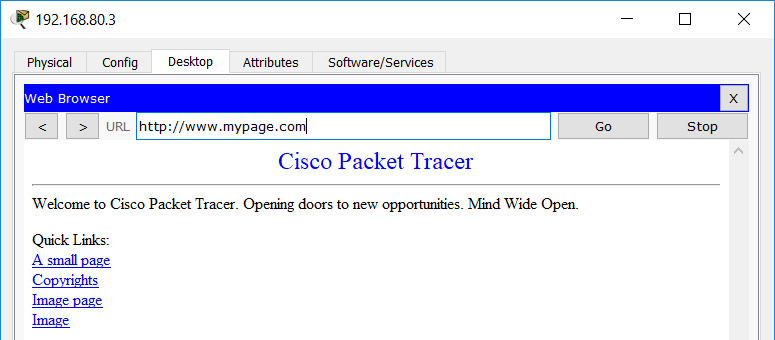
\includegraphics[width=.9\textwidth]{img/192_168_80_3__1}
\end{center}
Средствами встроенного браузера, была открыта страница сайта \textbf{www.mypage.com}, которая была предварительно автоматически сгенерирована.
\end{frame}


\begin{frame}[fragile]
\frametitle{Проверка TFTP}
На Router 2 была открыта консоль, в которой были выполнены следующие команды:
\begin{lstlisting}[language={}]
Router>enable
Router#show flash

System flash directory:
File  Length   Name/status
  3   5571584  pt1000-i-mz.122-28.bin
  2   28282    sigdef-category.xml
  1   227537   sigdef-default.xml
[5827403 bytes used, 58188981 available, 64016384 total]
63488K bytes of processor board System flash (Read/Write)

Router#copy flash tftp
Source filename []? pt1000-i-mz.122-28.bin
Address or name of remote host []? 192.168.120.1
Destination filename [pt1000-i-mz.122-28.bin]? temp.file

Writing pt1000-i-mz.122-28.bin...!!!!!!!!!!!!!!!!!!!!!!
[OK - 5571584 bytes]

5571584 bytes copied in 0.147 secs (8684467 bytes/sec)
\end{lstlisting}
\end{frame}


\begin{frame}[fragile]
\frametitle{Проверка TFTP}
Разберем действия:
\begin{enumerate}
\item Командой \textbf{enable} был совершен переход в привелегированный режим, можно заметить по символу решетки;
\item Командой \textbf{show flash} было выведено содержимое флеш-памяти, в данном случае это необходимо для тестовой загрузки по TFTP;
\item Командой \textbf{copy flash tftp} сообщаем о начале загрузке файла по tftp, где далее указывается файл(ы), tftp сервер для загрузки, а также новое имя файла(ов). 
\end{enumerate}
\end{frame}


\begin{frame}
\frametitle{Проверка TFTP}
Как и ожидалось, на сервере, в настройках TFTP появился выбранный ранее файл с указанным именем.
\begin{center}  
	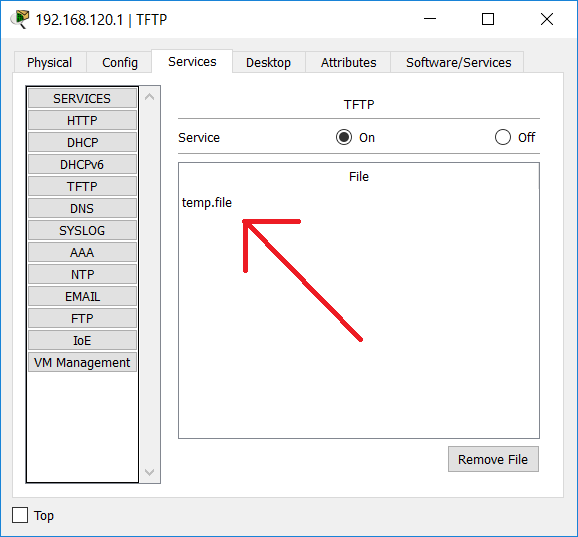
\includegraphics[width=.9\textwidth]{img/192_168_120_1__2}
\end{center}
\end{frame}


\begin{frame}
\frametitle{Проверка с помощью Traffic Sumulator}
\begin{center}  
	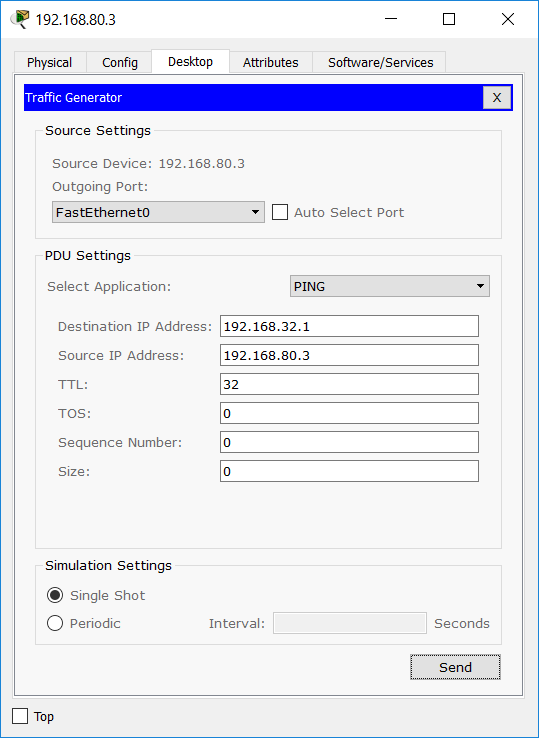
\includegraphics[width=.5\textwidth]{img/traffic_0}
\end{center}
\end{frame}


\begin{frame}
\frametitle{Проверка с помощью Traffic Sumulator}
С помощью утилиты Traffic Sumulator можно выполнять разнообразные сетевые команды с выбранными настройками.

Также имеется возможность, по шагам проследить за пакетами.
\begin{center}  
	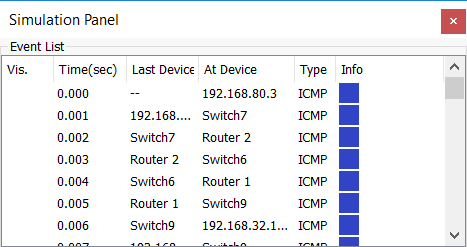
\includegraphics[width=.6\textwidth]{img/traffic_1}
\end{center}
\end{frame}



%\begin{frame}[fragile]
%\frametitle{Проверка первичного и вторичного DNS сервером}
%На первичном сервере вводим команду \textbf{cat /etc/log/syslog}
%\begin{lstlisting}[language={}]
%...
%... zone example.com/IN: loaded serial 1
%... zone 40.168.192.in-addr.arpa/IN: loaded serial 1
%... zone 255.in-addr.arpa/IN: loaded serial 1
%... zone localhost/IN: loaded serial 2
%... all zones loaded
%... running
%... zone 40.168.192.in-addr.arpa/IN: sending notifies (serial 1)
%...
%\end{lstlisting}
%Как видно из части лога, зоны были успешно загружены и переданы на вторичный сервер.
%\end{frame}


\begin{frame}[fragile]
\frametitle{Вывод}
В данной работе был получен опыт по работе в \textbf{Cisco Packet Tracer}.

По сравнению с прошлыми работами, где построение происходило с помощью WMware, в данном случае сеть была построена и настроена гораздо быстрее.

Построение и настройка были выполнены с помощью встроенных инструментов, которые в общем виде имитируют реальное оборудование. Если сравнивать с WMware, то в нем были рассмотрена настройка сети на конкретных системах(FreeBSD, NetBSD), в то время как в Cisco Packet Tracer это было сделано на лишь приближенных к реальности устройствах.

В общем случае Cisco Packet Tracer будет полезен при проектировании сети, но даст не так много опыта как WMware при настройке реальных систем.
\end{frame}	
	

	
\end{document}
